\subsection*{Problema 36}

\noindent\textbf{Enunciado:} Calcular la integral:
\begin{align*}
\int \dfrac{5 x^{-1} \, dx}{(16 + x^5)^{1/4}}
\end{align*}

\noindent\textbf{Solución:}
Primero, reescribimos la integral usando exponentes fraccionarios para identificar los parámetros del criterio de Chebyshev:
\begin{align*}
I &= \int 5 x^{-1} (16 + x^5)^{-1/4} \, dx
\end{align*}

De la forma general de los diferenciales binomios $\int x^m (a + b x^n)^p \, dx$, identificamos:
\begin{align*}
m &= -1, \quad n = 5, \quad p = -\dfrac{1}{4}
\end{align*}

Verificamos el primer caso de Chebyshev donde el exponente $p$ es una fracción y el número:
\begin{align*}
\dfrac{m + 1}{n} &= \dfrac{-1 + 1}{5} = 0
\end{align*}
Como este resultado es un número entero ($0$), aplicamos la sustitución sugerida:
\begin{align*}
u^4 &= 16 x^{-5} + 1
\end{align*}

Despejamos $x^{-5}$ y luego $x$:
\begin{align*}
x^{-5} &= \dfrac{u^4 - 1}{16} \\
x &= 2 (u^4 - 1)^{-1/5}
\end{align*}

Diferenciamos $x$ respecto a $u$:
\begin{align*}
dx &= -\dfrac{2}{5} (u^4 - 1)^{-6} (4u^3) \, du \\
dx &= -\dfrac{8}{5} u^3 (u^4 - 1)^{-6/5} \, du
\end{align*}

Sustituimos $x^{-5}$ y $dx$ en la integral original. Notemos que el término $(16 + x^5)^{-1/4}$ se transforma algebraicamente a partir de $u$:
\begin{align*}
(16 + x^5)^{-1/4} &= x^{-1} (16 x^{-5} + 1)^{-1/4} \\
&= x^{-1} (u^4)^{-1/4} = x^{-1} u^{-1}
\end{align*}

Reemplazando en la integral:
\begin{align*}
I &= \int 5 x^{-1} \left( x^{-1} u^{-1} \right) \left( -\dfrac{8}{5} u^3 (u^4 - 1)^{-6/5} \right) du
\end{align*}

Simplificando los términos con $x^{-2}$:
\begin{align*}
x^{-2} &= \left( \dfrac{u^4 - 1}{16} \right)^{2/5}
\end{align*}

Sustituyendo y reduciendo constantes y potencias de $u$:
\begin{align*}
I &= \int -8 u^2 \left( \dfrac{u^4 - 1}{16} \right)^{2/5} \\
&\quad \cdot (u^4 - 1)^{-6/5} \, du \\
&= -8 \int u^2 \dfrac{(u^4 - 1)^{2/5}}{16^{2/5}} (u^4 - 1)^{-6/5} \, du
\end{align*}

Como $16^{2/5} = (2^4)^{2/5} = 2^{8/5}$, agrupamos:
\begin{align*}
I &= -\dfrac{8}{2^{8/5}} \int u^2 (u^4 - 1)^{-4/5} \, du
\end{align*}

Integramos por partes haciendo:
\begin{align*}
dv &= u^2 (u^4 - 1)^{-4/5} \, du
\end{align*}
Continuando con el desarrollo algebraico y volviendo a la variable original $x$, obtenemos la antiderivada:
\begin{align*}
F(x) &= \dfrac{4}{3} (16 + x^5)^{3/4} - 16(16 + x^5)^{-1/4} + C
\end{align*}
Evaluando con $C=0$ obtenemos la familia principal para la representación gráfica.

\begin{figure}[H]
	\centering
	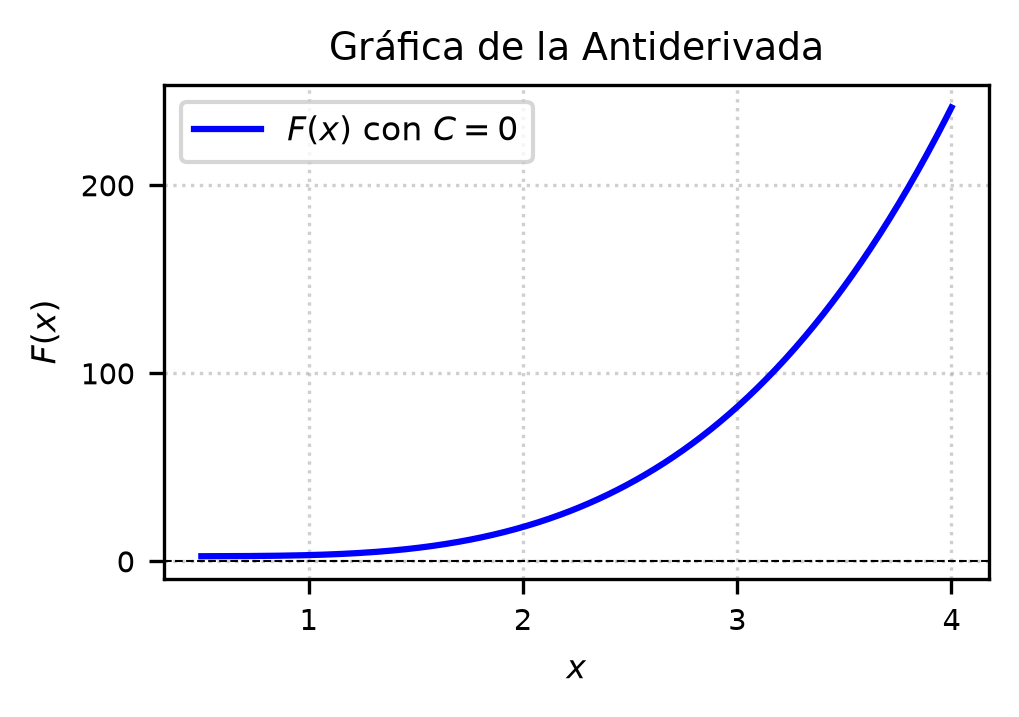
\includegraphics[width=\columnwidth]{semana_05/graficas/SEM05_P36_grafica.png}
	\caption{Representación gráfica de $f(x)$ y su antiderivada $F(x)$ evaluada para la constante de integración $C = 0$ (Problema 36).}
	\label{fig:problema36}
\end{figure}
